\chapter{Architecture}

\section{Overview}
\begin{figure}[h!]
	\centering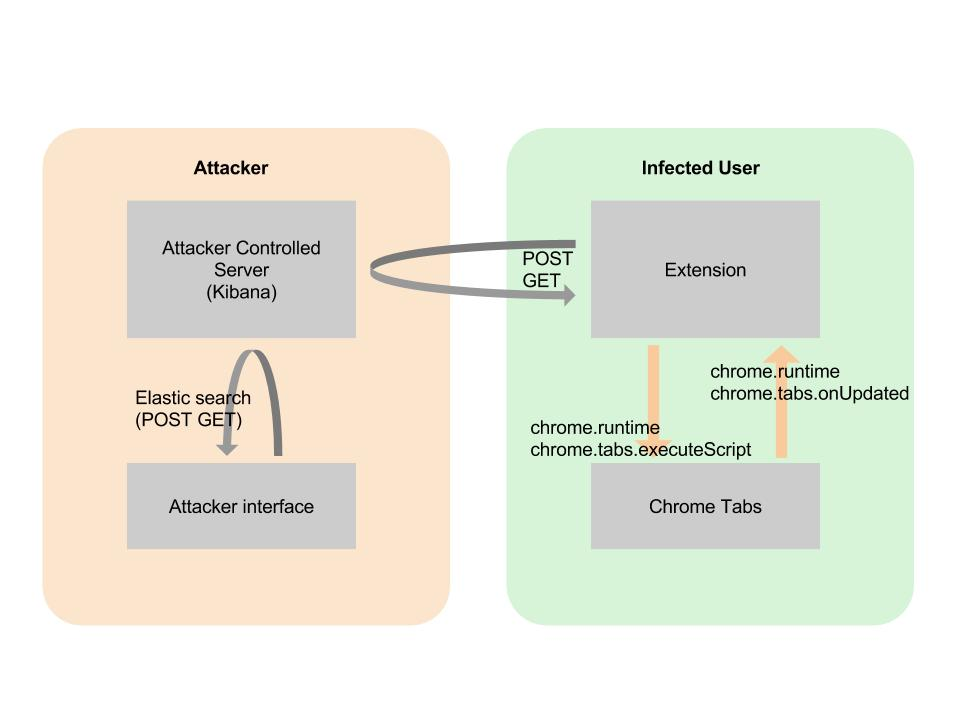
\includegraphics[width=\textwidth,height=\textheight,keepaspectratio]{architecture1.jpg}
	\caption{Architecture Overview}
	\label{fig:1}
\end{figure}

\subsection{Explanation} 
The system can be divide in to two major parts, the client or victim side and the server or attacker side. The client has the extension installed on his/her browser which keeps track of every required events or actions being performed by the user on the browser tabs. The extension then sends the information to an attacker controlled server (Kibana in our case) via network requests, which stores all the data received. The attacker has control to this server and can pull/push data to it using a REST interface.

\section{Database Schema}
\begin{figure}[h!]
	\centering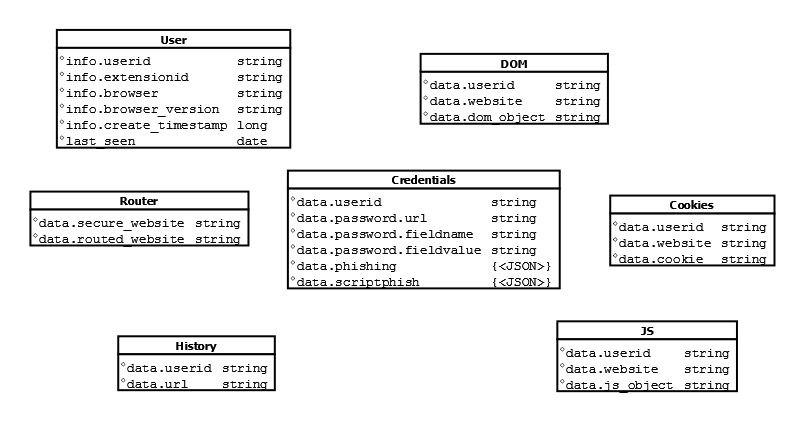
\includegraphics[width=\textwidth,height=\textheight,keepaspectratio]{DB.png}
	\caption{Schema}
	\label{fig:2}
\end{figure}

\subsection{Database Schema Overview}
\subsubsection{User Table}
The table stores all the informational data about a user, such as the unique user ID, the extension ID on their system, the Browser used, Broswer Version, extension installation timestamp and the last time the user was seen/online. 

\subsubsection{Router}
This table maintains a global list of security websites and the link they should be rerouted to, if an user visits any of these links. The table is user agnostic. 

\subsubsection{History}
This table maintains the History of each user in the form of a time stamp and the link visited as key value pairs. 

\subsubsection{Credentials}
This maintains all the stolen credentials of each user by the client side.

\subsubsection{Cookies}
Similar to credentials, this one stores all the stolen cookies.

\subsubsection{DOM}
This is a table of all the DOM objects that can be inserted in the user's webpage and is stored in the form strings per userID and weblink combination.

\subsubsection{JS}
Similar to DOM, this has the Javascript objects in form of strings to be injected to user webpages.